\documentclass[12pt,
               a4paper, 
               english,          % Hifenizacoes em ingles
               brazil            % Ultimo idioma é o padrao do documento
               ]{report}
\usepackage[brazil]{babel}   
\usepackage[top=3cm,
            bottom=2cm,
            left=3cm,
            right=2cm]{geometry}
\usepackage[T1]{fontenc}		% Selecao de codigos de fonte.
\usepackage[utf8]{inputenc}		% Codificacao do documento (conversão 
\usepackage{PTSerif}             % Opções de fontes em: https://ctan.org/topic/font
\usepackage{graphicx}		    % Inclusão de gráficos
\usepackage{lscape}             % usado para rotacionar tabelas, etc
\usepackage{adjustbox}
\usepackage{color}
\usepackage{microtype} 			% para melhorias de justificação
\usepackage[indentfirst=false]{quoting} % utilizadao para folha de rosto e epigrafe
\usepackage{setspace} % utilizado para alterar o espacamento em determinadas paginas do texto
\usepackage{url}
\usepackage{enumitem} % Utilizada para formatar uma lista enumerada 
\usepackage{booktabs}
\usepackage{arydshln}
\usepackage{tocloft} % Utilizada para customizar cabecalho e lista de figuras e tabelas
\usepackage{float}


\usepackage{lipsum} %pode remover quando for realizar o trabalho

%%%%%% REDEFININDO LOCAL DA PAGINACAO - INICIO %%%%%%%%%%%%%%%%%%%%%%%%
\usepackage{fancyhdr} % Pacote utilizado para alterar a posicao da paginação
\pagestyle{fancy}
\fancyhf{} % Limpa todos os cabeçalhos e rodapés padrão
\fancyhead[R]{\thepage} % Coloca o número da página no canto superior direito
\renewcommand{\headrulewidth}{0pt} % Remove a linha do cabeçalho (opcional)
\fancypagestyle{plain}{
    \fancyhf{} % Limpa cabeçalhos e rodapés
    \fancyhead[R]{\thepage} % Número da página no canto superior direito
    \renewcommand{\headrulewidth}{0pt} % Remove a linha do cabeçalho
}
%%%%%% REDEFININDO LOCAL DA PAGINACAO - FIM %%%%%%%%%%%%%%%%%%%%%%%%

\onehalfspacing

\begin{document}

\addtocounter{page}{-2} % Diminuindo a paginacao em dois, para deconsiderar a capa e a ficha catalografica

%Dados usados em todo o documento
\makeatletter
\newcommand{\cidade}[1]{\gdef\@cidade{#1}}
\newcommand{\faculdade}[1]{\gdef\@faculdade{#1}}
\newcommand{\faculdadesigla}[1]{\gdef\@faculdadesigla{#1}}
\newcommand{\instcomp}[1]{\gdef\@instcomp{#1}}
\newcommand{\instnce}[1]{\gdef\@instnce{#1}}
\newcommand{\instncecurto}[1]{\gdef\@instncecurto{#1}}
\newcommand{\programa}[1]{\gdef\@programa{#1}}
\newcommand{\progsigla}[1]{\gdef\@progsigla{#1}}
\newcommand{\orientadora}[1]{\gdef\@orientadora{#1}}
\newcommand{\coorientadora}[1]{\gdef\@coorientadora{#1}}
\newcommand{\orientadorastitulo}[1]{\gdef\@orientadorastitulo{#1}}


\title{Titulo Completo do Trabalho}
\author{Nome do(a) Autor(a) do Trabalho}
\date{2025}
\cidade{Rio de Janeiro}
\faculdade{Universidade Federal do Rio de Janeiro}
\faculdadesigla{UFRJ}
\instcomp{Instituto de Computação}
\instnce{Instituto Tércio Pacitti de Aplicações e Pesquisas Computacionais}
\instncecurto{Instituto Tércio Pacitti de Aplicações}
\programa{Programa de Pós-Graduação em Informática}
\progsigla{PPGI}
\orientadora{Nome do(a) Orientador(a)}
\coorientadora{Nome do(a) Co-orientador(a)}
\orientadorastitulo{D.SC}
\makeatother

%Includes pré-textuais
\thispagestyle{empty}
\newgeometry{top=4cm,bottom=1cm,left=3cm,right=3cm}
\makeatletter
\begin{center}

\includesvg[width=1\textwidth]{figuras/logo_capa.svg}

\vspace{3cm}
\Large \@author

\vspace{2cm}
\Large \textbf{\MakeUppercase{\@title}}

\vspace*{\fill}
\@cidade\\
\@date

\end{center}
\makeatother
\restoregeometry
\newpage


\thispagestyle{empty}
\makeatletter
\begin{spacing}{1}
\begin{center}

\large \MakeUppercase{\@faculdade}

\large \MakeUppercase{\@instcomp}

\large \MakeUppercase{\@instnce}

\large \MakeUppercase{\@programa} (\@progsigla)

\vspace{2cm}
\large \MakeUppercase{\@author}

\vspace{2cm}
\large \textbf{\MakeUppercase{\@title}}
\end{center}

\vspace{0.5cm}
\begin{quoting}[leftmargin=7.5cm, rightmargin=1cm]
Dissertação de Mestrado apresentada ao \@programa, \@instcomp\ e  \@instnce, \@faculdade, como requisito parcial à obtenção do título de Mestre em Informática.
\end{quoting}

\vspace{2cm}
Orientadora: Profa. \@orientadora, \@orientadorastitulo

Co-orientadora: Profa. \@coorientadora, \@orientadorastitulo

\vspace*{\fill}
\begin{center}
\@cidade\\
\@date
\end{center}

\end{spacing}
\makeatother
\newpage

\thispagestyle{empty}
\newgeometry{top=18cm}
\begin{center}

\large CIP - Catalogação na Publicação

\end{center}
\restoregeometry
\newpage

\thispagestyle{empty}
\makeatletter
\begin{spacing}{1}
\begin{center}

\large \textbf{\@title}

\vspace{1.5cm}
\large \@author

\end{center}

\vspace{0.5cm}

\begin{quoting}[leftmargin=7.0cm, rightmargin=1cm]
Dissertação de Mestrado submetida ao \@programa\ do \@instcomp\ e do \@instncecurto\ da \@faculdade\ - \@faculdadesigla, como parte dos requisitos necessários à obtenção do título de Mestre em Informática.
\end{quoting}

\vspace{1.5cm}
Aprovado em 30 de março de 2025 por:

\vspace{2cm}
\begin{flushright}

\hspace{5cm} \hrulefill

Prof(a). \@orientadora, \@orientadorastitulo, \@progsigla/\@faculdadesigla (Presidente)

\vspace{2cm}
\hspace{5cm} \hrulefill

Prof(a). \@coorientadora, \@orientadorastitulo, \@progsigla/\@faculdadesigla

\vspace{2cm}
\hspace{5cm} \hrulefill

Prof(a). Nome do Representante da Banca, \@orientadorastitulo, NCE/\@faculdadesigla


\vspace{2cm}
\hspace{5cm} \hrulefill

Prof(a). Nome do Representante da Banca, \@orientadorastitulo, \@progsigla/\@faculdadesigla

\end{flushright}

\end{spacing}
\makeatother
\newpage

\thispagestyle{empty}
\begin{spacing}{1}
\vspace*{\fill}
\begin{quoting}[leftmargin=6.5cm, rightmargin=1cm]
Dedico esse trabalho ao meus pais, por todo amor, dedicação e compreensão. Amo vocês.  
\end{quoting}
\end{spacing}
\newpage


\thispagestyle{empty}
\makeatletter
\begin{center}
\textbf{\MakeUppercase{Agradecimentos}}
\end{center}


\lipsum[1-4]


\makeatother
\newpage

\thispagestyle{empty}
\begin{spacing}{1}
\vspace*{\fill}
\begin{quoting}[leftmargin=6cm, rightmargin=1cm]

\textit{``Descrever o texto da citacao utilizada na epígrafe.\\
O texto pode ter mais de uma linha caso se deseje. \\
Ou pode ser em um texto longo também. de acordo com a nacessidade e com a escolha feita.``\\}
(Nome do Autor)
\end{quoting}
\end{spacing}
\newpage






\thispagestyle{empty}
\begin{center}
\textbf{\MakeUppercase{Resumo}}
\end{center}

\lipsum[5]

\vspace{1em}

Palavras-chave: palavras; chaves; separadas; por; ponto e vírgula
\newpage

\thispagestyle{empty}
\begin{center}
\textbf{\MakeUppercase{Abstract}}
\end{center}

\lipsum[6]

\vspace{1em}

Keywords: key; words; separated; by; semi commas
\newpage

%Removendo inicialização da contagem de figuras por capitulo
\counterwithout{figure}{chapter}

%Define o formato do nome da figura
\renewcommand{\cftfigpresnum}{Figura~} 
\renewcommand{\cftfigaftersnum}{ - }
\renewcommand{\cftfignumwidth}{4.5em}

%Altera o titulo da lista de figuras
\renewcommand{\listfigurename}{Lista de Figuras}

%Formata o titulo da lista de figuras
\renewcommand{\cftloftitlefont}{\hfill\bfseries\MakeUppercase} % Centraliza o título e deixa em negrito
\renewcommand{\cftafterloftitle}{\hfill} % Garante o alinhamento central

%imprime a lista de figiras
\listoffigures
\thispagestyle{empty} %remove a exibicao da pagina
\newpage

%Removendo inicialização da contagem de tabelas por capitulo
\counterwithout{table}{chapter}

%Define o formato do nome da tabela
\renewcommand{\cfttabpresnum}{Tabela~} 
\renewcommand{\cfttabaftersnum}{ - }
\renewcommand{\cfttabnumwidth}{4.5em}

%Altera e formata o titulo da lista de tabelas
\renewcommand{\listtablename}{\normalsize\centerline{\bfseries\MakeUppercase{Lista de Tabelas}}}


%imprime a lista de figiras
\listoftables
\thispagestyle{empty} %remove a exibicao da pagina
\newpage

\thispagestyle{empty}
\begin{center}
\textbf{\MakeUppercase{Lista de Abreviaturas e Siglas}}
\end{center}
\vspace{0.5cm}
\begin{spacing}{2}
\noindent
FSP - Feature Space Partition\\
IA - Inteligencia Artificial\\
ML - Machine Learning
\end{spacing}
\newpage

\addtocontents{toc}{\protect\thispagestyle{empty}} % força o "empty" na primeira pagina do sumário
\pagestyle{empty} % remove a nunemracao das demais paginas de sumario (se houver mais de uma) 

%apresenta ate o nivel 5, de paragrafo
\setcounter{tocdepth}{4}

%apresenta a numeracao ate o nivel 5, de paragrafo
\setcounter{secnumdepth}{4}

% titletoc 
\titlecontents{chapter}[10pt]
  {\normalfont\normalsize\bfseries}
  {\contentslabel{10pt}\uppercase} % removido \MakeUppercase
  {}
  {\titlerule*[0.4pc]{.}\contentspage} % aqui sim!

\titlecontents{section}[17pt]
  {\normalfont\normalsize}
  {\contentslabel{17pt}\uppercase}
  {}
  {\titlerule*[0.4pc]{.}\contentspage}

\titlecontents{subsection}[30pt]
  {\normalfont\normalsize\bfseries}
  {\contentslabel{30pt}}
  {}
  {\titlerule*[0.4pc]{.}\contentspage}

\titlecontents{subsubsection}[45pt]
  {\normalfont\normalsize\bfseries\itshape}
  {\contentslabel{45pt}}
  {}
  {\titlerule*[0.4pc]{.}\contentspage}

\titlecontents{paragraph}[53pt]
  {\normalfont\normalsize\itshape}
  {\contentslabel{53pt}}
  {}
  {\titlerule*[0.4pc]{.}\contentspage}


%Altera e Formata o titulo do sumario
\renewcommand{\contentsname}{\vspace{-65pt}\normalsize\centerline{\bfseries\MakeUppercase{Sumário}}}

\tableofcontents % Insere o sumário
\clearpage % Garante que o sumário termine aqui
\pagestyle{fancy} % Retorna ao estilo "fancy" para o restante do documents

%Includes p do texto principal
\chapter{Introdução}

Como exposto em \cite{Torralba2008}, o aprendizado de máquina tem sido utilizado como alternativa à implementação de algoritmos específicos e complexos durante a resolução de diversos tipos de problemas. 

\lipsum[6]

A Figura \ref{fig:mlapplications}, apresenta um breve resumo das possíveis aplicações do aprendizado de máquina.

\begin{figure}[ht]
    \centering
    \caption{Domínio de aplicações do aprendizado de máquina.}
    \copyrightbox[b]
    		{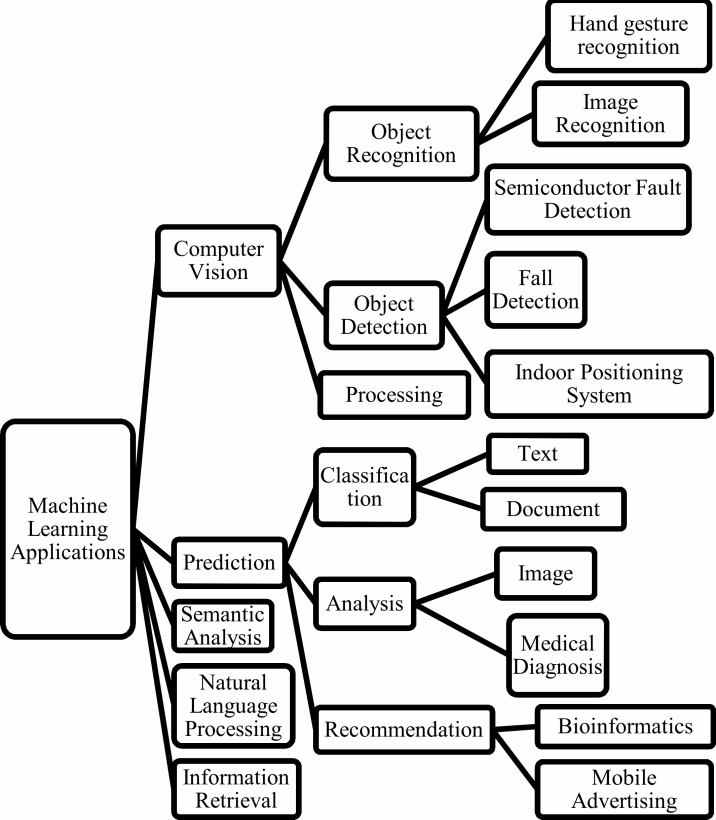
\includegraphics[width=0.7\linewidth]{mlapplications}}
            {Fonte: Extraída de \cite{ApplicationMachineLearning}}
    \label{fig:mlapplications}
\end{figure}

\lipsum[7-8]

\section{Motivação}

Como apresentado em \cite{MLBigdata}, com o resultado do desenvolvimento das tecnologias web, das redes sociais e dispositivos móveis, ocorreu uma verdadeira explosão no crescimento dos dados. 

\lipsum[9-16]


\section{Categorização do problema}

\lipsum[17-18]

\section{Proposta do trabalho}

\lipsum[19-21]

\section{Estrutura dessa trabalho}

O restante deste texto está organizado da seguinte forma. A Seção~\ref{cap:referencial_teorico} apresenta os conceitos básicos do referencial teórico necessário para um melhor entendimento do trabalho, com a apresentação dos assuntos tal, tal e tal. A Seção~\ref{cap:trabalhos_relacionados} contextualiza outros trabalhos que realizaram trabalhos similares. A Seção~\ref{cap:proposta_de_pesquisa} lista as questões da pesquisa, bem como seu objetivo principal e concluindo com as contribuições esperadas com o resultado final do trabalho. A Seção~\ref{cap:metodologia} demonstra qual foi a metodologia do trabalho. A Seção~\ref{cap:experimentos} explica como os experimentos foram executados. A Seção~\ref{cap:resultados} apresenta os resultados dos experimentos, Pot fim a Seção~\ref{cap:conclusao} apresenta um sumário dos resultados e sugestões para trabalhos futuros. 

\chapter{Referencial teórico}
\label{cap:referencial_teorico}

Essa seção apresenta um pequeno conjunto de assuntos considerados pré-requisitos para um melhor entendimento desse trabalho.

\lipsum[22]

\section{Assunto 1 do referencial teórico} \label{sub:assunto2}

\lipsum[23-27]

\section{Assunto 2 do referencial teórico}

\lipsum[23-27]

\begin{enumerate}
    \item Exemplo de litstagem enumerada;
    \item Outro exemplo de de litstagem enumerada;
    \item Último exemplo de listagem enumerada.
\end{enumerate}

\lipsum[28]:

\begin{itemize}
    \item Exemplo de listagem com bullets;
    \item Outro exemplo de listagem com bullets; 
    \item Exemplo final de listagem com bullets. 
\end{itemize}


\chapter{Trabalhos relacionados}\label{cap:trabalhos_relacionados}

\lipsum[30-36]

\chapter{Proposta de pesquisa}\label{cap:proposta_de_pesquisa}

Essa seção apresenta tanto as questões de pesquisa que norteiam a necessidade da mesma, bem como os objetivos primário e específicos relacionados ao trabalho.

\section{Questões de pesquisa} \label{sub:questpesq}

As perguntas que devem %pretendem 
ser respondidas ao final deste trabalho são apresentadas a seguir:

\begin{enumerate}
    \item Qual a primeira pergunta de pesquisa do trabalho?
    %\item É possível paralelizar o método FSP utilizando a linguagem Python?
    \item Qual seria outra pergunta de pesquisa do trabalho?
    \item Ainda tem mais pergunta de pesquisa para colocar aqui?
\end{enumerate}

\section{Objetivo principal}

O principal objetivo deste trabalho de pesquisa é "Descrever qual o principal objetivo deste trabalho de pesquisa".


\section{Contribuições esperadas}
As principais contribuições esperadas como resultado deste trabalho são:

\begin{enumerate}
    \item Primeira contribuição esperada do trabalho;
    \item Segunda contribuição esperada do trabalho;
    \item Colocar quantas contribuições quiser.
\end{enumerate}

\chapter{Metodologia}\label{cap:metodologia}

Essa seção apresenta a metodologia a ser adotada no trabalho.

Segue um exemplo de link externo em uma nota de rodape. Foi criado um DOI para identificar univocamente essa implementação. A ferramenta Zenodo foi utilizada para essa finalidade. O DOI criado foi o 10.5281/zenodo.15048153 \footnote{A última versão dessa implementação pode ser acessada em: \url{https://doi.org/10.5281/zenodo.15048153}}.

\lipsum[37-38]

\begin{figure}[ht]
    \centering
    \caption{Processo iterativo usado no desenvolvimento}
    \copyrightbox[b]
  		{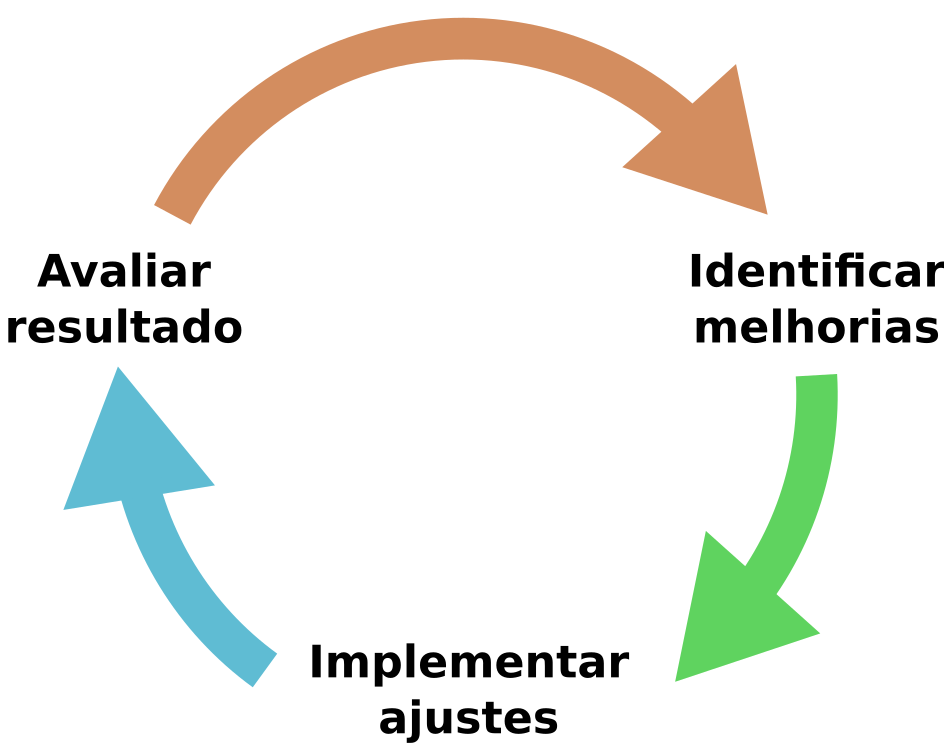
\includegraphics[width=0.4\linewidth]{metodologia}}
        {Fonte: O autor (2025)}
    \label{fig:metodologia}
\end{figure}

\lipsum[39-41]

\chapter{Desenvolvimento do trabalho}\label{cap:desenvolvimento_trabalho}
Essa seção apresenta o que foi realizado no trabalho.

\lipsum[22]

\section{Assunto 1 do desenvolvimento do trabalho}
\lipsum[23-27]

\section{Assunto 2 do desenvolvimento do trabalho}

\lipsum[23-27]

\begin{enumerate}
    \item Exemplo de litstagem enumerada;
    \item Outro exemplo de de litstagem enumerada;
    \item Último exemplo de listagem enumerada.
\end{enumerate}

\lipsum[28]:

\begin{itemize}
    \item Exemplo de listagem com bullets;
    \item Outro exemplo de listagem com bullets; 
    \item Exemplo final de listagem com bullets. 
\end{itemize}


\chapter{Experimentos}\label{cap:experimentos}

Nesse capítulo será abordado o escopo dos experimentos, em qual ambiente foram executados, os detalhes dos datasets utilizados bem como a metodologia definida para a sua execução. 

\section{Ambiente utilizado}


\subsection{Configurações de hardware}

Os experimentos foram realizados utilizando a seguinte configuração de hardware:

\begin{itemize}
    \item Processador: Intel\textsuperscript{\tiny{\copyright}} Core\textsuperscript{\tiny{TM}} i9-13900KF 
    \begin{itemize}
        \item Núcleos: 20
        \item Threads: 32
        \item Velocidade: 5.40GHz
    \end{itemize}
    \item Memória RAM: 64 GB
    \item SSD M2: 1.8 TB
    \item Placa de vídeo: NVIDIA GeForce RTX 4060, 8GB
\end{itemize}

\subsection{Configurações de software}

Os seguintes configurações e componentes de software foram utilizados durante a sua execução:

\begin{itemize}
    \item Sistema Operacional: Linux Mint 22, kernel 6.8.0-41-generic
    \item Python (3.12.8) 
    \item Conda (24.11.3) 
    \item Matplotlib (3.9)
\end{itemize}

\section{Exemplo de Section do experimento}

\lipsum[7]

\subsection{Exemplo de subsection do experimento}

\lipsum[8]
A Tabela \ref{tab:tabelaexemplo1}, apresenta as informações \lipsum[9]

Foram descartadas as observações que possuíam valores nulos, e os atributos que não não eram do tipo numérico.  
\begin{table}[H]
\caption{Exemplo de tabela de uso genérico}
\begin{center}
\fontsize{10pt}{13pt}\selectfont
\begin{tabular}{lcccc}
\toprule
                  Base de dados & Observações  &   Features   &   Classe      & Desbalanceamento\\
                                & (used/total) & (used/total) & (used/total)  &                 \\
\midrule
                       Dataset1 &   150/150    &     4/4      &     3/3       & 1.00            \\
                       Dataset3 &   208/208    &    60/60     &     2/2       & 1.14            \\
                       Dataset3 &   214/214    &     9/10     &     6/7       & 8.44            \\
\bottomrule
\multicolumn{5}{l}{Fonte: O autor (2025)}
\end{tabular}
\label{tab:tabelaexemplo1}
\end{center}
\end{table}


\subsubsection{Exemplo de subsubsection do experimento}

\lipsum[10-12]


\chapter{Resultados}\label{cap:resultados}

Essa seção presenta os resultados do experimento \lipsum[11]

\section{Resultados do experimento}

\lipsum[12-13]

Na Tabela \ref{tab:resultados} foram tabulados todos os dados de resultados das execuções dos experimentos. 

A tabela apresenta uma listagem \lipsum[14]

\lipsum[15-17]

\subsection{Análise dos resultados}
Ao avaliar os dados da Tabela \ref{tab:resultados}, é possível realizar algumas observações de cunho mais geral:

\lipsum[18]


\begin{landscape}
\begin{table}
\caption{Exemplo de tabela complexa e rotacionada}
\fontsize{10pt}{13pt}\selectfont
\begin{tabular}{lcccccc}
\toprule
Dataset                       & Tipo processamento  & Tempo Treinamento (s) &   Tempo Predict1 (s)   &    Tempo Predict2 (s)  &  Acurácia1    &  Acurácia2    \\
\midrule
Nome Dataset1                 & Serial              &     2.03 (0.06)       &  0.0287 (0.005281)     & 0.0237 (0.000715)      &  94.24 (1.41) & 94.71 (1.24)  \\
\cdashline{2-7}[1pt/1pt]
                              & CPU Multi-thread    &     2.44 (0.06)       &  0.0272 (0.000206)     & 0.0240 (0.000617)      &  93.22 (0.91) & 93.93 (1.17)  \\
\cdashline{2-7}[1pt/1pt]
                              & GPU                 &     3.00 (0.13)       &  0.0279 (0.000537)     & 0.0244 (0.000725)      &  93.31 (1.64) & 94.22 (1.43)  \\
\midrule 
Nome Dataset1                 & Serial              &    29.47 (0.28)       &  0.0718 (0.000702)     & 0.1673 (0.005537)      &  85.26 (1.67) & 84.04 (2.29)  \\
\cdashline{2-7}[1pt/1pt]
                              & CPU Multi-thread    &    36.02 (0.39)       &  0.0705 (0.000369)     & 0.1670 (0.005399)      &  86.36 (1.69) & 84.41 (1.45)  \\
\cdashline{2-7}[1pt/1pt]
                              & GPU                 &    40.04 (0.40)       &  0.0703 (0.000834)     & 0.1507 (0.004985)      &  85.80 (1.18) & 84.28 (1.68)  \\
\midrule 
Nome Dataset2                 & Serial              &    70.27 (0.65)       &  0.0575 (0.000698)     & 0.2215 (0.003645)      &  67.91 (1.97) & 69.91 (1.62) \\
\cdashline{2-7}[1pt/1pt]
                              & CPU Multi-thread    &    83.12 (0.74)       &  0.0577 (0.000530)     & 0.2403 (0.004444)      &  68.40 (1.84) & 69.88 (2.01) \\
\cdashline{2-7}[1pt/1pt]
                              & GPU                 &    97.14 (0.76)       &  0.0571 (0.000587)     & 0.2162 (0.003746)      &  67.66 (1.76) & 69.50 (1.95) \\
\midrule 
Nome Dataset4                 & Serial              &   340.85 (1.36)       &  0.2050 (0.001077)     & 0.6914 (0.014545)      &  80.06 (1.24) & 79.96 (1.40) \\
\cdashline{2-7}[1pt/1pt]
                              & CPU Multi-thread    &   396.73 (2.19)       &  0.2020 (0.001227)     & 0.6844 (0.012787)      &  80.59 (1.16) & 80.54 (1.12) \\
\cdashline{2-7}[1pt/1pt]
                              & GPU                 &   440.27 (2.22)       &  0.2022 (0.001252)     & 0.6848 (0.012288)      &  80.34 (1.03) & 79.85 (1.26) \\
\midrule 
Nome Dataset5                 & Serial              &   463.12 (2.26)       &  0.1283 (0.001132)     & 0.6212 (0.012257)      &  70.69 (1.96) & 70.84 (1.64) \\
\cdashline{2-7}[1pt/1pt]
                              & CPU Multi-thread    &   542.16 (3.25)       &  0.1263 (0.000826)     & 0.6240 (0.012652)      &  69.71 (1.53) & 70.30 (1.41) \\
\cdashline{2-7}[1pt/1pt]
                              & GPU                 &   621.60 (3.05)       &  0.1320 (0.001443)     & 0.7037 (0.015179)      &  70.06 (1.83) & 70.12 (1.62) \\
\midrule 
Nome Dataset6                 & Serial              &   823.81 (112.64)     &  0.0178 (0.000912)     & 19.6347 (0.541860)     &  82.14 (0.27) & 82.94 (0.26) \\
\cdashline{2-7}[1pt/1pt]
                              & CPU Multi-thread    &   805.33 (79.41)      &  0.0150 (0.000670)     & 18.8484 (0.485823)     &  82.15 (0.26) & 82.97 (0.29) \\
\cdashline{2-7}[1pt/1pt]
                              & GPU                 &   962.65 (126.90)     &  0.0307 (0.001097)     & 16.7377 (0.473457)     &  82.16 (0.30) & 82.91 (0.29) \\
\midrule 
Nome Dataset7                 & Serial              & 10986.52 (162.84)     &  0.1610	(0.007035)    &107.2397	(1.481285)	  &  77.06 (0.30) & 80.48 (0.25) \\
\cdashline{2-7}[1pt/1pt]
                              & CPU Multi-thread    & 10832.09 (140.02)     &  0.1586	(0.006309)    &106.4547	(1.219125)	    &  77.07 (0.40) & 80.35 (0.30) \\
\cdashline{2-7}[1pt/1pt]
                              & GPU                 & 11762.89 (157.42)     &  0.1595	(0.006406)    &107.8366	(1.210092)	    &  77.04 (0.28) & 80.44 (0.33) \\
\bottomrule
\multicolumn{7}{l}{Fonte: O autor (2025)}
\end{tabular}
\label{tab:resultados}
\end{table}
\end{landscape}
\newpage

\chapter{Conclusão}\label{cap:conclusao}

\lipsum[20-24]

%Includes pós-textuais
\renewcommand{\bibname}{\normalsize\centerline{\bfseries\uppercase{Referências}}}

\addcontentsline{toc}{chapter}{REFERÊNCIAS} % Adiciona a bibliografia ao índice

\bibliographystyle{abntex2-alf}
\bibliography{3-pos-textuais/bibi}

\end{document}
